\question (南京理工大学,1996年)有一组数据(15,9,7,8,20,-1,7,4),用堆排序的筛选方法建立的初始堆为(
)
\par\fourch{-1,4,8,9,20,7,15,7}{-1,7,15,7,4,8,20,9}{\textcolor{red}{-1,4,7,8,20,15,7,9}}{A,B,C均不对}
\begin{solution}将堆的数组还原为完全二叉树,根据堆的含义表明,完全二叉树中所有非终端结点的值均不大于(或不小于)其左右孩子结点的值,本题只有C选项符合。
\end{solution}
\question (华中科技大学,2006年)构建n个记录的初始堆,其时间复杂度为( )
\par\fourch{\textcolor{red}{}}{}{}{}
\begin{solution}初始化堆只需要遍历一遍全部元素即可,因此时间复杂度为O(n)。
\end{solution}
\question (南京邮电大学,2004年)从堆中删除一个元素的时间复杂度为( )
\par\fourch{}{\textcolor{red}{}}{}{}
\begin{solution}从堆中删除一个元素,我们把堆中最后的元素填入删除元素的位置,然后向下调整,这个调整的时间复杂度为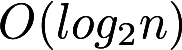
\includegraphics[width=0.65625in,height=0.18750in]{texmath/39368f5Cdpi7B3507DO28log_2n29}。
\end{solution}
\question (重庆大学,2004年)对于序列(32,47,12,8,2,19,30),其堆顶元素最小的初始堆是(
)
\par\fourch{\textcolor{red}{(2,8,12,32,47,19,30)}}{(2,8,12,19,30,32,47)}{(2,12,8,32,19,47,30)}{(2,12,8,30,19,32,47)}
\begin{solution}序列(32,47,12,8,2,19,30)对应的最小堆调整过程如下图所示:
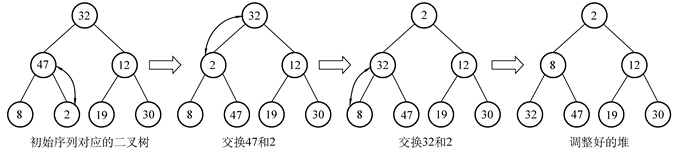
\includegraphics[width=7.07292in,height=1.59375in]{computerassets/960c7c52cb71db72b4c086f278de7ace.jpeg}
因此,最后结果为(2,8,12,32,47,19,30)。 【堆调整过程】
从无序序列所确定的完全二叉树的第一个非叶子结点开始,从右至左,从下至上,对每个结点进行调整,最终将得到一个小顶堆。
\end{solution}
\question 已知关键序列5,8,12,19,28,20,15,22是小根堆(最小堆),插入关键字3,调整后得到的小根堆是(
)
\par\fourch{\textcolor{red}{3,5,12,8,28,20,15,22,19}}{3,5,12,19,20,15,22,8,28}{3,8,12,5,20,15,22,28,19}{3,12,5,8,28,20,15,22,19}
\begin{solution}插入关键字3的过程如下图所示。
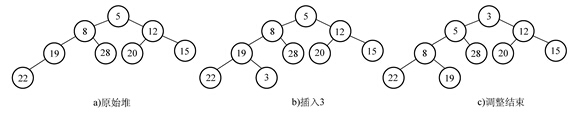
\includegraphics[width=5.85417in,height=1.18750in]{computerassets/2442b2878aef21035ef5b347f9b1bdcf.jpeg}
\end{solution}
\question 已知序列25,13,10,12,9是大根堆,在序列尾部插入新元素18,将其再调整为大根堆,调整过程中元素之间进行的比较次数是(
~)
\par\twoch{1}{\textcolor{red}{2}}{4}{5}
\begin{solution}对堆插入或删除一个元素,有可能不满足堆的性质,堆被破坏,需要调整为新堆。

(1)为原堆,

(2)为插入18后,

(3)比较10与18,交换后,

(4)比较25与18,不交换,即为调整后的新的大根堆。

因此调整过程中元素之间进行的比较次数为2。

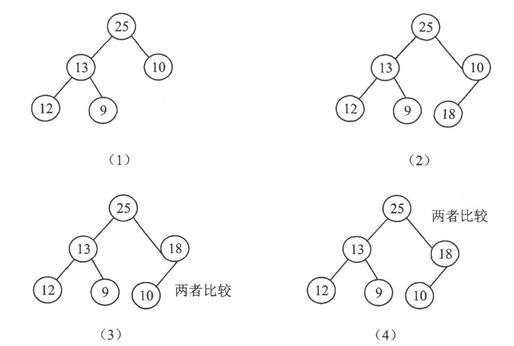
\includegraphics[width=3.33333in,height=2.23958in]{computerassets/fbd0f5bd21064b67a7bed1e8b35715bf.png}
\end{solution}
\question 已知小根堆为8,15,10,21,34,16,12,删除关键字8
之后需重建堆,在此过程中, 关键字之间的比较数是( )
\par\twoch{1}{\textcolor{red}{2}}{3}{4}
\begin{solution}最小堆的概念和最小堆的重建。
\end{solution}
\question (西南交通大学,2005年)下面的序列中( )序列是堆
\par\fourch{\textcolor{red}{1,2,8,4,3,9,10,5}}{1,5,10,6,7,8,9,2}{9,8,7,6,4,8,2,1}{9,8,7,6,5,4,3,7}
\begin{solution}A是一个小顶堆
\end{solution}
\question (中山大学,2005年)一个无序序列12,36,41,20,80,55采用顺序表存储表示,采用堆排序算法建立的初始(大顶)堆是(
)
\par\fourch{80,12,55,20,36,41}{80,36,20,12,55,41}{\textcolor{red}{80,36,55,20,12,41}}{80,12,55,20,36,41}
\begin{solution}ABD都不满足构成堆的条件
\end{solution}
\question (中国科学技术大学,2004年)查找低效的数据结构是( )
\par\twoch{有序顺序表}{二叉排序树}{\textcolor{red}{堆}}{平衡二叉树}
\begin{solution}堆的查找复杂度是O(n),其他的几个是O(logn),因为堆并不是单纯为查找而设计的数据结构
\end{solution}
\question (南京林业大学,2005年)堆是一种有用的数据结构。以下关键字序列(
)是一个堆
\par\fourch{16,72,31,23,94,53}{94,23,31,72,16,53}{16,53,23,94,31,72}{\textcolor{red}{16,23,53,31,94,72}}
\begin{solution}16,23,53,31,94,72是一个小顶堆
\end{solution}
\question (武汉大学,2004年)下面4个序列中,只有( )满足堆的定义
\par\fourch{\textcolor{red}{49,38,42,15,38,19,13,12}}{49,12,42,38,24,13,19,38}{49,42,19,13,38,24,38,12}{49,42,19,38,38,24,13,12}
\begin{solution}A是一个大顶堆
\end{solution}
\question (南京邮电大学,2004年)从堆中删除一个元素的时间复杂度为( )
\par\twoch{O(1)}{\textcolor{red}{O(logn)}}{O(n)}{O(nlogn)}
\begin{solution}从堆中删除一个元素,我们把堆中最后的元素填入删除元素的位置,然后向下调整,这个调整的时间复杂度为O(logn)
\end{solution}
